\section{$\mathcal{\mathcal{C} \mskip -4mu \mathcal{E}}$ Machine} \label{sec:mach}

Using the calculus of cactus environments defined in the previous section, we
derive an abstract machine: the $\mathcal{\mathcal{C} \mskip -4mu \mathcal{E}}$ machine. The syntax
and semantics are defined in Figure~\ref{fig:CEM}. 

\begin{figure*}
\textbf{Syntax}
\begin{align*}
\tag{State} s &::= \langle c, \sigma, \mu \rangle \\
\tag{Term} t &::= i \; | \; \lambda t \; | \; t \; t  \\
\tag{Variable} i &\in \mathbb{N}  \\
\tag{Closure} c &::= t [l] \\
\tag{Value} v &::= \lambda t[l] \\
\tag{Heap} \mu &::= \epsilon \; | \; \mu [ l \mapsto \rho ] \\
\tag{Environment} \rho &::= \bullet \; | \; c \cdot l \\
\tag{Context} \sigma &::= \square \; | \; \sigma \; c \;  | \; \sigma \; u \\
\tag{Location} l,u,f &\in \mathbb{N}
\end{align*}
\textbf{Semantics}
\begin{align*}
\tag{Upd}
\langle v,  \sigma \; u , \mu[u \mapsto c \cdot l] \rangle 
  &\rightarrow_{\mathcal{\mathcal{C} \mskip -4mu \mathcal{E}}}
\langle v, \sigma, \mu[u \mapsto v \cdot l] \rangle  \\
\tag{Lam}
\langle \lambda t[l], \sigma \; c, \mu \rangle 
  &\rightarrow_{\mathcal{\mathcal{C} \mskip -4mu \mathcal{E}}}
\langle t[f], \sigma, \mu[f \mapsto c \cdot l]\rangle f \not \in \textnormal{dom}(\mu)  \\
\tag{App}
\langle t \; t'[l], \sigma, \mu \rangle
  &\rightarrow_{\mathcal{\mathcal{C} \mskip -4mu \mathcal{E}}}
\langle t[l], \sigma \; t'[l], \mu \rangle \\
\tag{Var1}
\langle 0[l], \sigma, \mu \rangle
  &\rightarrow_{\mathcal{\mathcal{C} \mskip -4mu \mathcal{E}}}
\langle c, \sigma \; l , \mu \rangle 
\; \textnormal{where} \; c \cdot l' = \mu(l)\\
\tag{Var2}
\langle i[l], \sigma, \mu \rangle
  &\rightarrow_{\mathcal{\mathcal{C} \mskip -4mu \mathcal{E}}}
\langle (i-1)[l'], \sigma, \mu \rangle
\; \textnormal{where} \; c \cdot l' = \mu(l)
\end{align*}
\caption{Syntax and semantics of the $\mathcal{\mathcal{C} \mskip -4mu \mathcal{E}}$ machine.}
\label{fig:CEM}
\end{figure*}

The machine operates on a similar syntax as the calculus, extended only with a
context to implement the updates from the NVar subderivation ($\sigma \; u$) and
the operands from the NEval subderivation ($\sigma \; c$). On the update rule,
the current closure is a value, and there is an update marker as the outermost
context. This implies that a variable was entered and that the current closure
represents the corresponding value for that variable. Thus, we update the
location $u$ that the variable entered, replacing whatever term was entered
with the current closure. The Lam rule takes an argument off the context and
binds it to a variable, allocating a fresh heap location for the bound
variable. This ensures that every instance of the variable will point to this
location, and thus the bound term will be evaluated at most once. The App rule
simply pushes an argument term in the current environment. The Var1 rule enters
the closure pointed to by the environment location, while the Var2 rule
traverses the cactus environment to locate the correct closure.  

To get some intuition for the $\mathcal{\mathcal{C} \mskip -4mu \mathcal{E}}$
machine and how it works, consider the depiction in Figure~\ref{fig:state} of
its state during evaluation of the term: $(\lambda a.(\lambda b.b \; a)
(\lambda c.c \; a)) ((\lambda i.i) (\lambda j.j))$. We leave the variable names
for readability. For thoroughness, the occurrences of variable $a$ may be
replaced with index $1$, and the rest can be replaced with index $0$. At this
point in the computation, the closure for $a$ is shared, and has been updated
with its value. The closure in the context (the $a$ from the application $c
\; a$) now points to the updated value.

\begin{figure}
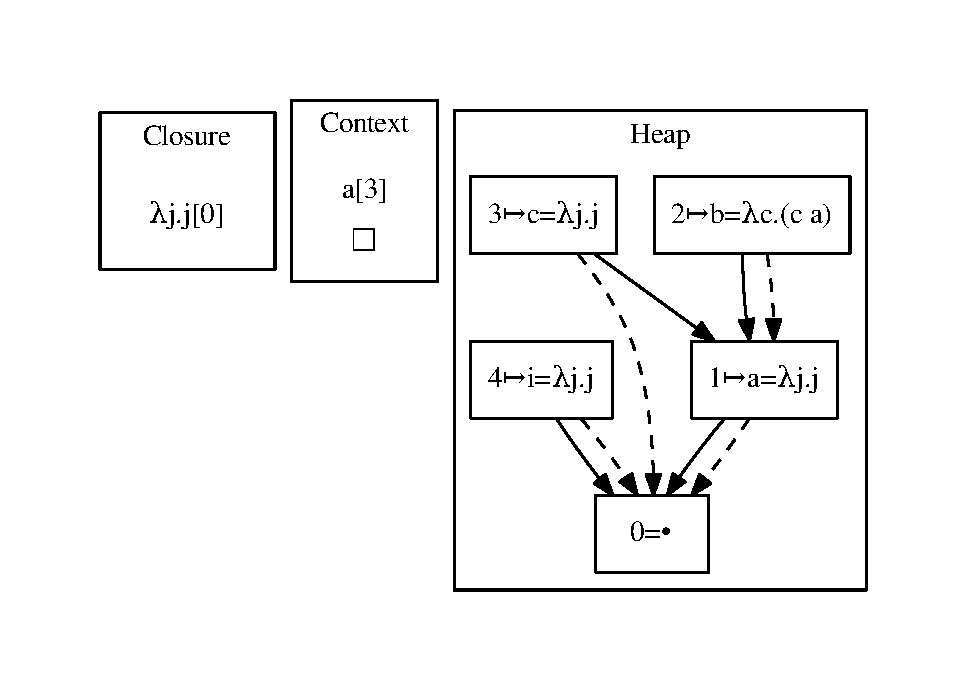
\includegraphics[width=\linewidth]{figures/18.pdf}

\caption{$\mathcal{\mathcal{C} \mskip -4mu \mathcal{E}}$ machine state example.
The dotted lines represent the environment for the bound closure, and the solid
lines represent the next environment cell:  $t[dotted] \cdot solid$.  Variables
are left in for readability, but can be trivially replaced with deBruijn
indices.  }
\label{fig:state}
\end{figure}

\subsection{Correctness}
We prove that the reflexive transitive closure of the $\mathcal{\mathcal{C} \mskip -4mu \mathcal{E}}$ machine
step relation evaluates to a value and heap and empty context iff
$\xrightarrow{}_{N}$ evaluates to the same value and heap.

{\theorem \textnormal{(Equivalence)} $$(c, \mu) \rightarrow_{N} (v, \mu') \;
\leftrightarrow \; \langle c, \square, \mu \rangle \xrightarrow{*
}_{\mathcal{\mathcal{C} \mskip -4mu \mathcal{E}}} \langle v, \square, \mu' \rangle $$} 

By induction on the $\rightarrow_{N}$ step relation and the reflexive transitive
closure of the $\rightarrow_{\mathcal{\mathcal{C} \mskip -4mu \mathcal{E}}}$ step relation.

